\aberturaModulo{UNIDADE III}{PROJETOS E VIABILIDADE}{Encontros 12 a 14 $\bullet$ Base da AV2 (20\%) e Engenharia Financeira da AV3}{%
Esta unidade converte a estratégia territorial e o modelo de negócios da Unidade II em engenharia econômica e modelagem financeira auditável. Ao longo de três encontros e um simulado quantitativo, o estudante aprende a estruturar projetos executivos de investimento, decidir sua localização territorial com rigor multicritério, projetar fluxos de caixa livres, aplicar métricas de viabilidade sob risco e estimar o valor econômico de empreendimentos tecnológicos e de impacto.
\begin{itemize}[leftmargin=1.4em, itemsep=3pt]
  \item \textbf{Capítulo 12: Elaboração de Projetos de Investimento e Decisão Locacional:} ciclo do projeto (Woiler \& Mathias, 2008), fatores locacionais clássicos (Weber, Von Thünen), Matriz Locacional Ponderada, orçamento de CAPEX, Ciclo Financeiro / Capital de Giro (NLCG), OPEX e Ponto de Equilíbrio Contábil.
  \item \textbf{Capítulo 13: Métodos e Ferramentas para Análise de Investimentos:} valor do dinheiro no tempo, Fluxo de Caixa Livre (FCL), VPL, TIR (e suas anomalias), MTIR, VAUE para vidas úteis distintas, Payback Simples e Descontado, análise de sensibilidade e cenários.
  \item \textbf{Capítulo 14: Valuation de Empreendimentos Tecnológicos e Projetos de Impacto:} preço versus valor, Fluxo de Caixa Descontado (Damodaran, 2010), WACC, perpetuidade de Gordon, Enterprise Value e Equity Value, \textit{Dark Side of Valuation}, Método de Venture Capital e Opções Reais.
  \item \textbf{Simulado III: Preparatório Quantitativo da AV2 (20\%):} 8 questões objetivas de cálculo integral (A--E), 2 estudos dirigidos dissertativos, gabarito passo a passo, espelho e diagnóstico.
\end{itemize}
}

\chapter{Elaboração de Projetos de Investimento e Decisão Locacional}
\label{cap:12}

\noindent\tagAV{AV2 (20\%)}\ \tagQuant\ \tagTerritorio
\vspace{6pt}

\begin{capObjetivos}
Ao concluir este capítulo, você será capaz de:
\begin{enumerate}[leftmargin=1.4em, itemsep=2pt]
  \item Estruturar a passagem da ideia empreendedora ao projeto executivo de investimento segundo o ciclo de estudo de mercado, engenharia, localização e orçamento (Woiler \& Mathias, 2008).
  \item Avaliar alternativas territoriais combinando fatores locacionais clássicos (Weber e Von Thünen), infraestrutura energética e hídrica, densidade de P\&D e incentivos fiscais por meio da \textbf{Matriz Locacional Ponderada}.
  \item Dimensionar a estrutura orçamentária completa de um projeto: investimento fixo (\textbf{CAPEX}), Necessidade Líquida de Capital de Giro (\textbf{NLCG}) derivada do ciclo financeiro e custos operacionais (\textbf{OPEX}).
  \item Calcular e interpretar o \textbf{Ponto de Equilíbrio Contábil} (em unidades e em receita) e a margem de segurança operacional diante de variações locacionais e tributárias.
\end{enumerate}
\end{capObjetivos}

\begin{capRevisao}
Antes de avançar para a modelagem orçamentária e locacional, relembre três fundamentos das Unidades I e II:
\begin{itemize}[leftmargin=1.4em, itemsep=2pt]
  \item \textbf{Aglomerações e Eficiência Coletiva (Cap. 2):} a localização não é apenas custo de frete; proximidade a fornecedores especializados, universidades e mão de obra qualificada gera economias externas que reduzem custos unitários e aceleram o aprendizado tecnológico.
  \item \textbf{Proposta de Valor e Estrutura de Custos no Canvas (Cap. 9):} todo bloco de atividades-chave e recursos-chave do modelo de negócios precisa ser traduzido em imobilizações (CAPEX) e despesas recorrentes (OPEX) para que o empreendimento saia do plano discursivo.
  \item \textbf{Instrumentos de Fomento Regional (Cap. 10):} linhas como BNB/FNE, BNDES, FINEP e FAPESB financiam parcelas distintas do projeto (máquinas, obras, P\&D ou capital de giro), exigindo separação contábil clara entre investimento fixo e giro.
\end{itemize}
\end{capRevisao}

\etapa{3}{Fundamentação Teórica, Fatores Locacionais e Orçamento do Projeto}

\subsection{Da ideia ao projeto executivo (Woiler \& Mathias, 2008)}

Uma ideia tecnológica ou territorialmente enraizada só se torna financiável quando convertida em um \textbf{projeto de investimento}, isto é, um conjunto sistematizado de informações técnicas, mercadológicas, locacionais, jurídicas e econômico-financeiras que permite decidir se vale a pena imobilizar recursos escassos hoje em troca de benefícios futuros incertos. Na tradição brasileira de elaboração e análise de projetos sistematizada por Woiler e Mathias (2008), essa trajetória percorre três estágios progressivos de redução de incerteza, nos quais cada etapa filtra riscos antes de comprometer capital em engenharia dispendiosa.

No estágio inicial de \textbf{Identificação da Oportunidade e Estudo de Pré-Viabilidade}, você delimita o problema territorial ou tecnológico, estima a demanda potencial (TAM/SAM/SOM) e verifica restrições legais ou ambientais eliminatórias antes de gastar com engenharia detalhada. Superada essa triagem preliminar, o \textbf{Anteprojeto ou Estudo de Viabilidade Técnica e Econômica (EVTE)} define a escala de produção, a tecnologia de processo, a localização ótima, o cronograma físico-financeiro, o orçamento de CAPEX, Capital de Giro e OPEX, além das projeções de fluxo de caixa que sustentam a decisão de investir. Por sua vez, o \textbf{Projeto Executivo (Final)} detalha plantas arquitetônicas, memoriais descritivos de equipamentos, especificações elétricas e hidráulicas, contratos de fornecimento e licenças ambientais definitivas, servindo de base direta para contratação de obras e liberação de crédito junto a bancos de fomento.

\begin{boxSimbolo}[Vocabulário Conceitual e Símbolos do Capítulo 12]
Na modelagem locacional, $w_i$ representa o peso atribuído ao critério $i$ na Matriz Locacional Ponderada ($\sum_{i=1}^{m} w_i = 1$), $n_{ij}$ indica a nota atribuída à localidade candidata $j$ no critério $i$ em escala padronizada (por exemplo, de $0$ a $10$), e $Nota_j$ corresponde à pontuação global ponderada da localidade $j$. Na teoria clássica de Weber, $IM$ designa o Índice Material, definido como a razão entre o peso dos insumos localizados transportados e o peso do produto acabado.

Na estrutura orçamentária, \textbf{CAPEX} (\textit{Capital Expenditure}) refere-se ao investimento fixo em ativos de longo prazo (terrenos, obras civis, máquinas, equipamentos, licenças e softwares imobilizados), enquanto \textbf{OPEX} (\textit{Operational Expenditure}) reúne as despesas e os custos recorrentes necessários para manter a operação funcionando (matéria-prima, energia, salários, manutenção, fretes e aluguel). O dimensionamento do giro utiliza $PME$, $PMR$ e $PMP$, que correspondem respectivamente ao Prazo Médio de Estocagem, ao Prazo Médio de Recebimento de vendas e ao Prazo Médio de Pagamento a fornecedores (em dias), originando o Ciclo Financeiro ($CF_{ciclo}$, em dias) e a Necessidade Líquida de Capital de Giro ($NLCG$, em \reais{}). Para a análise de equilíbrio operacional, $CF$ representa os Custos e Despesas Fixas totais no período (em \reais{}), $P$ o preço unitário de venda, $CV_u$ o custo variável unitário, $MC_u = P - CV_u$ a margem de contribuição unitária e $PE$ o Ponto de Equilíbrio Contábil.
\end{boxSimbolo}

\subsection{Fatores locacionais clássicos e contemporâneos}

A escolha de onde implantar uma unidade produtiva, laboratório ou centro de distribuição altera permanentemente a estrutura de custos e a capacidade de inovação do negócio. A teoria econômica espacial oferece dois marcos clássicos que dialogam diretamente com os fatores contemporâneos de base tecnológica.

\begin{boxConceito}[Teoria Locacional Clássica: Von Thünen e Alfred Weber]
\textbf{Johann Heinrich von Thünen (1826: Renda da Terra e Distância ao Mercado)} analisou como o custo de transporte até o centro consumidor determina o uso ótimo do solo agrícola em anéis concêntricos. Produtos perecíveis ou de frete caro por unidade de valor ocupam áreas próximas ao mercado, ao passo que atividades extensivas de baixo custo de transporte deslocam-se para a periferia.

\textbf{Alfred Weber (1909: Triângulo Locacional e Índice Material)} formulou a localização industrial de mínimo custo de transporte entre fontes de matéria-prima e mercado consumidor. Quando o processo produtivo perde muito peso (matéria-prima bruta volumosa gerando produto leve e concentrado, isto é, $IM > 1$), a fábrica tende a se localizar \textbf{junto à fonte de matéria-prima}, caracterizando a orientação à matéria-prima típica de beneficiamento mineral, celulose e agroindústrias como fécula de mandioca ou desfibramento de sisal. Quando o produto ganha peso ou volume no envase ou montagem (como bebidas engarrafadas com água local), a fábrica orienta-se \textbf{para o mercado consumidor}.
\end{boxConceito}

Em empreendimentos tecnológicos e agroindustriais contemporâneos no Brasil, especialmente no Nordeste e na Bahia, a decisão locacional amplia a análise do frete ao incorporar seis vetores territoriais decisivos. O primeiro vetor envolve os \textbf{custos de transporte e logística multimodal}, medidos pela distância a rodovias duplicadas, ferrovias como a FIOL, portos como Salvador, Aratu e Ilhéus, além da qualidade das vias vicinais de escoamento. O segundo vetor trata da \textbf{infraestrutura energética e hídrica}, abrangendo disponibilidade de rede trifásica estável, tarifas industriais, irradiação solar e segurança hídrica para processos industriais ou de bioeconomia no Semiárido. O terceiro vetor corresponde à \textbf{densidade de P\&D e capital humano}, traduzida na proximidade a universidades (como UEFS, UFBA, UFRB, UNEB e SENAI CIMATEC), institutos tecnológicos e oferta de técnicos e engenheiros.

A esses elementos somam-se os \textbf{incentivos fiscais e fundiários}, como redução de ICMS estadual, isenção de IPTU e ISS municipal, cessão de terrenos em distritos industriais e acesso a fundos constitucionais (FNE/SUDENE). A \textbf{aglomeração setorial e a rede de fornecedores} em Arranjos Produtivos Locais (APLs) também pesam na escolha, pois reduzem custos de manutenção, peças de reposição e serviços especializados. Todo esse conjunto permanece condicionado às \textbf{restrições ambientais e de licenciamento}, que exigem compatibilidade com o zoneamento ecológico-econômico, outorga d'água e distanciamento de áreas de preservação permanente. A Figura~\ref{fig:12_ciclo} ilustra como o ciclo de elaboração de projetos articula esses vetores locacionais à estrutura orçamentária do empreendimento.

\begin{figure}[H]
  \centering
  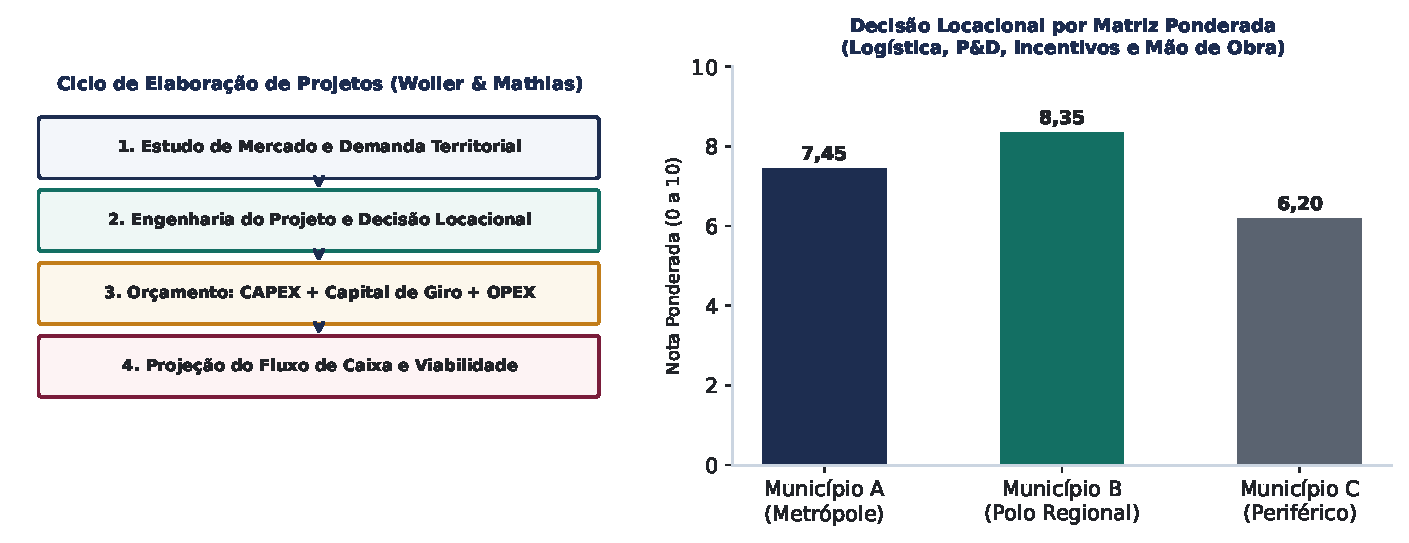
\includegraphics[width=0.95\textwidth]{figures/fig12_ciclo_projetos_localizacao.pdf}
  \caption{Ciclo de elaboração de projetos de investimento, vetores locacionais e integração orçamentária (CAPEX, Capital de Giro e OPEX).}
  \label{fig:12_ciclo}
\end{figure}

\subsection{Matriz Locacional Ponderada}

Quando múltiplos critérios qualitativos e quantitativos competem entre si, o projetista utiliza a \textbf{Matriz Locacional Ponderada} (método de pontuação compensatória). O procedimento exige definir pesos normalizados que reflitam a estratégia do negócio e atribuir notas comparáveis a cada município ou distrito candidato.

\begin{boxFormula}[Matriz Locacional Ponderada]
\[
  Nota_j = \sum_{i=1}^{m} w_i \cdot n_{ij}, \qquad \text{com} \quad \sum_{i=1}^{m} w_i = 1
\]
Para aplicar a matriz com rigor, inicia-se pela definição dos critérios eliminatórios e classificatórios, descartando previamente locais sem licença ambiental viável ou energia mínima exigida. Em seguida, atribuem-se os pesos ($w_i$), distribuindo $1{,}00$ ($100\%$) entre os $m$ critérios conforme o impacto econômico-tecnológico no projeto. Cada localidade $j$ recebe então uma pontuação ($n_{ij}$) em escala uniforme (por exemplo, $0$ a $10$) com base em dados objetivos como tarifas, distância em quilômetros e alíquotas. Multiplica-se $w_i \cdot n_{ij}$ para cada critério e soma-se a coluna da localidade $j$, escolhendo o território de maior $Nota_j$ após verificar a sensibilidade do ranking a pequenas alterações de pesos.
\end{boxFormula}

\subsection{Estrutura Orçamentária: CAPEX, Capital de Giro e OPEX}

Todo projeto de investimento organiza suas saídas de caixa em três grandes blocos que exigem tratamento contábil e financeiro separado. O primeiro bloco é o \textbf{CAPEX (\textit{Capital Expenditure}, ou Investimento Fixo)}, que engloba aquisições de ativos imobilizados e intangíveis de vida útil superior a um ano, tais como terreno, terraplanagem, galpão industrial, máquinas, equipamentos de laboratório, instalações elétricas, veículos utilitários, patentes e softwares corporativos. Esse investimento sofre \textbf{depreciação} (ou amortização) contábil ao longo do tempo e é desembolsado principalmente no Ano $0$ ou em fases programadas de expansão.

O segundo bloco corresponde ao \textbf{Capital de Giro e à Necessidade Líquida de Capital de Giro (NLCG)}, representando o recurso financeiro mantido em circulação para sustentar o descasamento temporal entre pagar fornecedores, estocar insumos, produzir, vender e receber dos clientes. Mesmo um projeto altamente lucrativo perde solvência se falhar no financiamento de seu ciclo financeiro.

O terceiro bloco reúne o \textbf{OPEX (\textit{Operational Expenditure}, ou Custos e Despesas Operacionais)}, composto pelos gastos contínuos do dia a dia para operar a capacidade instalada. Esses gastos dividem-se em \textbf{Custos e Despesas Fixas ($CF$)}, que permanecem constantes diante de variações no volume produzido dentro da faixa de capacidade (aluguel, folha administrativa, depreciação contábil, seguro e vigilância), e \textbf{Custos Variáveis ($CV$)}, que crescem proporcionalmente às unidades produzidas e vendidas (matéria-prima direta, embalagens, energia de processo, comissões e impostos sobre venda).

\begin{boxFormula}[Ciclo Financeiro, NLCG e Ponto de Equilíbrio Contábil]
\textbf{1. Ciclo Financeiro e Necessidade Líquida de Capital de Giro:}
\[
  CF_{ciclo} = PME + PMR - PMP \qquad \Longrightarrow \qquad NLCG = CF_{ciclo} \times \frac{\text{OPEX desembolsável anual}}{360}
\]
onde $PME$ é o prazo médio de estocagem, $PMR$ o prazo médio de recebimento e $PMP$ o prazo médio de pagamento (em dias). Se $CF_{ciclo} > 0$, a empresa precisa financiar $NLCG$ em caixa; se $CF_{ciclo} < 0$, os fornecedores financiam a operação.

\vspace{6pt}
\textbf{2. Ponto de Equilíbrio Contábil ($PE$) e Margem de Segurança ($MS$):}
\[
  PE_{\text{unid}} = \frac{CF}{P - CV_u} = \frac{CF}{MC_u}, \qquad PE_{\text{receita}} = PE_{\text{unid}} \times P, \qquad MS(\%) = \frac{Q_{\text{prevista}} - PE_{\text{unid}}}{Q_{\text{prevista}}} \times 100\%
\]
onde $CF$ são os custos e despesas fixas do período, $P$ o preço unitário de venda, $CV_u$ o custo variável unitário e $MC_u = P - CV_u$ a margem de contribuição unitária. O $PE_{\text{unid}}$ indica o volume mínimo de vendas para que o lucro operacional (LAJIR) seja exatamente zero. Caso haja uma meta de lucro operacional $L_{\text{alvo}}$, soma-se $L_{\text{alvo}}$ ao numerador: $Q_{\text{meta}} = \frac{CF + L_{\text{alvo}}}{P - CV_u}$.
\end{boxFormula}

\etapa{4}{Exemplos Resolvidos Passo a Passo (Padrão de Engenharia Econômica)}

\begin{boxExemplo}{12.1}{Matriz Locacional Ponderada para Agroindústria no Território do Sisal}
\passoEnunciado{Uma cooperativa de inovação rural planeja instalar uma planta de extração de celulose e compósitos a partir de resíduo de sisal. Três municípios baianos foram pré-selecionados: Valente, Conceição do Coité e Feira de Santana.}
\passoDados{Critérios e pesos definidos pela equipe técnica: Proximidade à matéria-prima ($w_1 = 0{,}35$), Disponibilidade de energia e água ($w_2 = 0{,}25$), Infraestrutura logística e acesso a mercados ($w_3 = 0{,}25$) e Incentivos fiscais/terreno municipal ($w_4 = 0{,}15$). As notas técnicas de $0$ a $10$ foram: Valente $[9;\, 8;\, 7;\, 8]$, Conceição do Coité $[7;\, 8;\, 8;\, 7]$ e Feira de Santana $[6;\, 9;\, 9;\, 6]$.}
\passoPedido{Calcular a pontuação ponderada de cada município e indicar a localização recomendada.}
\passoMetodo{Aplicação direta da Matriz Locacional Ponderada: $Nota_j = \sum_{i=1}^{4} w_i \cdot n_{ij}$, verificando antes que $\sum w_i = 0{,}35 + 0{,}25 + 0{,}25 + 0{,}15 = 1{,}00$.}
\passoContas{%
\begin{align*}
  Nota_{\text{Valente}} &= (0{,}35 \times 9) + (0{,}25 \times 8) + (0{,}25 \times 7) + (0{,}15 \times 8) \\
  &= 3{,}15 + 2{,}00 + 1{,}75 + 1{,}20 = 8{,}10 \\[4pt]
  Nota_{\text{Coité}} &= (0{,}35 \times 7) + (0{,}25 \times 8) + (0{,}25 \times 8) + (0{,}15 \times 7) \\
  &= 2{,}45 + 2{,}00 + 2{,}00 + 1{,}05 = 7{,}50 \\[4pt]
  Nota_{\text{Feira}} &= (0{,}35 \times 6) + (0{,}25 \times 9) + (0{,}25 \times 9) + (0{,}15 \times 6) \\
  &= 2{,}10 + 2{,}25 + 2{,}25 + 0{,}90 = 7{,}50
\end{align*}
}
\passoResposta{O município selecionado é \textbf{Valente}, com nota global \textbf{8,10}, superando Conceição do Coité (7,50) e Feira de Santana (7,50) em 0,60 ponto.}
\passoVerificacao{A vantagem de Valente decorre do peso elevado da proximidade à matéria-prima ($35\%$), coerente com o Índice Material de Weber ($IM > 1$) para resíduos agrícolas volumosos: transportar talos e mucilagem bruta por longas distâncias até Feira de Santana destruiria a margem operacional.}
\end{boxExemplo}

\begin{boxExemplo}{12.2}{Dimensionamento de CAPEX Total e Capital de Giro pelo Ciclo Financeiro}
\passoEnunciado{Uma startup de sensores IoT para irrigação localizada no Oeste Baiano (Barreiras) está fechando seu orçamento de implantação para submissão ao FNE Inovação.}
\passoDados{Investimentos fixos previstos: galpão modular e bancadas técnicas \reais{180.000}, equipamentos de soldagem SMD e calibração \reais{220.000}, softwares e registro de firmware \reais{50.000}. Para a operação anual, o OPEX desembolsável projetado é de \reais{720.000}/ano (base comercial de $360$ dias). Os prazos médios negociados são: $PME = 30$ dias, $PMR = 45$ dias e $PMP = 25$ dias.}
\passoPedido{Calcular o CAPEX total, o Ciclo Financeiro ($CF_{ciclo}$), a Necessidade Líquida de Capital de Giro ($NLCG$) e o investimento inicial total requerido no Ano $0$.}
\passoMetodo{Soma dos ativos imobilizados para o CAPEX; cálculo de $CF_{ciclo} = PME + PMR - PMP$; conversão do ciclo em caixa pela taxa diária de desembolso ($\text{OPEX}/360$).}
\passoContas{%
\begin{align*}
  CAPEX &= 180.000 + 220.000 + 50.000 = \reais{450.000} \\[4pt]
  CF_{ciclo} &= 30 + 45 - 25 = 50\text{ dias} \\[4pt]
  \text{Desembolso diário} &= \frac{720.000}{360} = \reais{2.000/\text{dia}} \\[4pt]
  NLCG &= 50 \times 2.000 = \reais{100.000} \\[4pt]
  \text{Investimento Inicial Total} &= CAPEX + NLCG = 450.000 + 100.000 = \reais{550.000}
\end{align*}
}
\passoResposta{CAPEX = \textbf{\reais{450.000}}; Ciclo Financeiro = \textbf{50 dias}; NLCG = \textbf{\reais{100.000}}; Investimento Total no Ano 0 = \textbf{\reais{550.000}}.}
\passoVerificacao{O resultado faz pleno sentido econômico: embora o equipamento custe \reais{450.000}, a startup vende a prazo para produtores rurais ($45$ dias) e mantém estoque de componentes ($30$ dias) pagando fornecedores em $25$ dias, exigindo \reais{100.000} adicionais em caixa para não ficar insolvente nos primeiros meses.}
\end{boxExemplo}

\begin{boxExemplo}{12.3}{Ponto de Equilíbrio Contábil e Margem de Segurança em Bioinsumos}
\passoEnunciado{Uma biofábrica instalada no Recôncavo Baiano (Cruz das Almas) produz inoculantes biológicos líquidos em bombonas de 20 litros para agricultura familiar e médios produtores.}
\passoDados{Custos e despesas fixas anuais ($CF$) = \reais{180.000}; preço de venda por bombona ($P$) = \reais{120,00}; custo variável unitário ($CV_u$, incluindo meio de cultura, embalagem, comissão e imposto sobre venda) = \reais{75,00}; demanda anual contratada ($Q_{\text{prevista}}$) = $5.000$ bombonas.}
\passoPedido{Determinar a margem de contribuição unitária ($MC_u$), o Ponto de Equilíbrio em unidades ($PE_{\text{unid}}$) e em receita ($PE_{\text{receita}}$), além da Margem de Segurança ($MS$).}
\passoMetodo{Aplicação das equações de equilíbrio linear: $MC_u = P - CV_u$, $PE_{\text{unid}} = CF / MC_u$ e $MS = (Q_{\text{prevista}} - PE_{\text{unid}}) / Q_{\text{prevista}}$.}
\passoContas{%
\begin{align*}
  MC_u &= 120{,}00 - 75{,}00 = \reais{45{,}00/\text{bombona}} \\[4pt]
  PE_{\text{unid}} &= \frac{180.000}{45{,}00} = 4.000\text{ bombonas/ano} \\[4pt]
  PE_{\text{receita}} &= 4.000 \times 120{,}00 = \reais{480.000/\text{ano}} \\[4pt]
  MS(\%) &= \frac{5.000 - 4.000}{5.000} \times 100\% = \frac{1.000}{5.000} \times 100\% = 20\%
\end{align*}
}
\passoResposta{$MC_u = \mathbf{\reais{45{,}00}}$; $PE_{\text{unid}} = \mathbf{4.000\text{ bombonas}}$; $PE_{\text{receita}} = \mathbf{\reais{480.000}}$; Margem de Segurança = \textbf{20\%}.}
\passoVerificacao{Uma margem de segurança de $20\%$ indica que as vendas podem cair até $1.000$ bombonas abaixo do planejado antes que a biofábrica entre em prejuízo operacional. Esse colchão de segurança é coerente para agroindústrias expostas à sazonalidade climática.}
\end{boxExemplo}

\begin{boxExemplo}{12.4}{Orientação Locacional de Weber e Índice Material}
\passoEnunciado{Uma cooperativa de agricultores analisa onde instalar uma unidade de processamento de mandioca para produção de fécula seca: junto à zona produtora rural (Fonte), no meio do caminho (Entroncamento) ou na capital consumidora (Mercado).}
\passoDados{Para produzir $250\text{ t/ano}$ de fécula (produto acabado, PA), são necessárias $1.000\text{ t/ano}$ de raiz de mandioca bruta (matéria-prima, MP). A distância entre a fonte de MP e o mercado consumidor é de $100\text{ km}$. O frete rodoviário da MP custa \reais{2{,}00}$/(\text{t}\cdot\text{km})$ e o frete do PA custa \reais{3{,}00}$/(\text{t}\cdot\text{km})$.}
\passoPedido{Calcular o Índice Material ($IM$) de Weber e o custo total anual de transporte ($CT$) para as três localizações: na Fonte ($d_{MP}=0$, $d_{PA}=100$), no Entroncamento ($d_{MP}=50$, $d_{PA}=50$) e no Mercado ($d_{MP}=100$, $d_{PA}=0$).}
\passoMetodo{Cálculo de $IM = \text{Peso}_{MP} / \text{Peso}_{PA}$ e da função linear de custo de transporte $CT = Q_{MP} \cdot t_{MP} \cdot d_{MP} + Q_{PA} \cdot t_{PA} \cdot d_{PA}$.}
\passoContas{%
\begin{align*}
  IM &= \frac{1.000}{250} = 4{,}0 \quad (\text{perda de } 75\% \text{ de massa em água e casca}) \\[4pt]
  CT_{\text{Fonte}} &= (1.000 \times 2{,}00 \times 0) + (250 \times 3{,}00 \times 100) = 0 + 75.000 = \reais{75.000/\text{ano}} \\[4pt]
  CT_{\text{Entroncamento}} &= (1.000 \times 2{,}00 \times 50) + (250 \times 3{,}00 \times 50) = 100.000 + 37.500 = \reais{137.500/\text{ano}} \\[4pt]
  CT_{\text{Mercado}} &= (1.000 \times 2{,}00 \times 100) + (250 \times 3{,}00 \times 0) = 200.000 + 0 = \reais{200.000/\text{ano}}
\end{align*}
}
\passoResposta{$IM = \mathbf{4{,}0}$; a localização de menor custo de transporte é \textbf{na Fonte de matéria-prima} (\reais{75.000/ano}), gerando economia anual de \reais{125.000} em relação ao Mercado.}
\passoVerificacao{Mesmo com o frete unitário do produto acabado sendo $50\%$ mais caro que o da matéria-prima (\reais{3{,}00} contra \reais{2{,}00}), a redução de massa de $4$ para $1$ no beneficiamento torna economicamente irracional transportar água e resíduos brutos até a capital. Isso fundamenta a agroindustrialização descentralizada no interior.}
\end{boxExemplo}

\begin{boxExemplo}{12.5}{Análise de Trade-off: Incentivo Fiscal Territorial versus Custo Variável de Frete}
\passoEnunciado{Uma empresa de embalagens biodegradáveis avalia transferir sua planta da região metropolitana para um município do interior que oferece incentivos fiscais e fundiários, porém aumenta o custo de frete de entrega.}
\passoDados{Cenário Base (metropolitano): $CF = \reais{240.000/\text{ano}}$, $P = \reais{200{,}00/\text{unidade}}$ e $CV_u = \reais{120{,}00/\text{unidade}}$. Cenário Interior: cessão de galpão e isenção de taxas locais reduzem $CF$ em $25\%$, mas o frete adicional eleva $CV_u$ para \reais{128{,}00/\text{unidade}}.}
\passoPedido{Comparar o Ponto de Equilíbrio Contábil antes e depois da mudança locacional e avaliar se a transferência reduz o risco operacional.}
\passoMetodo{Cálculo de $PE_{\text{base}}$ e $PE_{\text{interior}}$ após atualização de $CF' = 0{,}75 \times CF$ e $CV_u' = 128{,}00$.}
\passoContas{%
\begin{align*}
  \text{Cenário Base:} \quad MC_u &= 200{,}00 - 120{,}00 = \reais{80{,}00}, \qquad PE_{\text{base}} = \frac{240.000}{80{,}00} = 3.000\text{ unidades} \\[6pt]
  \text{Cenário Interior:} \quad CF' &= 240.000 \times (1 - 0{,}25) = \reais{180.000} \\
  MC_u' &= 200{,}00 - 128{,}00 = \reais{72{,}00} \\
  PE_{\text{interior}} &= \frac{180.000}{72{,}00} = 2.500\text{ unidades}
\end{align*}
}
\passoResposta{O Ponto de Equilíbrio cai de \textbf{3.000 para 2.500 unidades/ano} (redução de $500$ unidades ou $16{,}7\%$), diminuindo o risco de prejuízo em cenários de baixa demanda.}
\passoVerificacao{O incentivo territorial compensa o frete adicional porque a redução de $25\%$ no custo fixo supera a perda de $10\%$ na margem de contribuição unitária. Acima de $7.500$ unidades ($60.000 / 8{,}00$), porém, o custo variável maior faria o cenário metropolitano gerar lucro total superior, evidenciando que a decisão depende da escala esperada.}
\end{boxExemplo}

\etapa{5}{Armadilhas Conceituais e Erros Mais Comuns}

\begin{boxErro}[Erro 1: Somar CAPEX e OPEX como se fossem despesas do mesmo período]
Incluir o valor integral de compra de máquinas (\reais{400.000} de CAPEX) dentro do custo fixo anual do Ponto de Equilíbrio distorce o cálculo, elevando artificialmente o $PE$. O ativo imobilizado entra no custo contábil anual apenas via \textbf{depreciação} (ou é tratado integralmente como investimento no Ano $0$ do Fluxo de Caixa Livre).
\end{boxErro}

\begin{boxErro}[Erro 2: Esquecer o Capital de Giro (NLCG) no investimento inicial]
Projetar apenas terrenos e máquinas e ignorar que a empresa precisa financiar estoques ($PME$) e vendas a prazo ($PMR$) leva à quebra de liquidez nos primeiros meses de operação, mesmo quando o produto tem boa margem de contribuição.
\end{boxErro}

\begin{boxErro}[Erro 3: Pesos não normalizados ou critérios redundantes na Matriz Locacional]
Atribuir pesos que não somam $1{,}00$ (ou $100\%$) ou duplicar o mesmo fator sob dois nomes diferentes (ex.: ``proximidade à rodovia'' e ``acesso rodoviário'') infla artificialmente um critério e invalida a comparação entre municípios.
\end{boxErro}

\begin{boxErro}[Erro 4: Confundir Ponto de Equilíbrio Contábil com Viabilidade Econômica]
Atingir o $PE_{\text{unid}}$ significa apenas que o lucro contábil operacional é zero, não que o projeto remunera o capital investido (TMA). Um projeto pode operar acima do Ponto de Equilíbrio e ainda assim destruir valor econômico se o retorno não superar o custo de oportunidade (Cap. 13).
\end{boxErro}

\etapa{6}{Lista de Exercícios de Fixação (15 Questões)}

\begin{enumerate}[leftmargin=1.6em, itemsep=5pt]
  \item Explique a diferença funcional entre estudo de pré-viabilidade, EVTE (anteprojeto) e projeto executivo segundo Woiler e Mathias (2008). \espacoResolucao[1.5cm]
  \item Por que uma agroindústria de processamento de polpa de frutas ou sisal tende a se localizar próxima à zona produtora, enquanto uma engarrafadora de refrigerantes tende a se localizar próxima ao mercado urbano? Utilize o conceito de Índice Material ($IM$) de Weber. \espacoResolucao[1.5cm]
  \item Uma empresa avalia dois municípios ($A$ e $B$) usando três critérios com pesos $w = [0{,}40;\, 0{,}30;\, 0{,}30]$. O Município $A$ obteve notas $[8;\, 7;\, 9]$ e o Município $B$ obteve $[9;\, 8;\, 6]$. Calcule as notas ponderadas e indique o vencedor. \espacoResolucao[1.6cm]
  \item Uma unidade de beneficiamento processa $500\text{ t/ano}$ de matéria-prima bruta para gerar $100\text{ t/ano}$ de produto acabado ($IM = 5$). A distância entre a fonte e o mercado é de $80\text{ km}$. O frete da MP custa \reais{1{,}50}$/(\text{t}\cdot\text{km})$ e o do PA custa \reais{2{,}50}$/(\text{t}\cdot\text{km})$. Compare o custo anual de transporte na Fonte versus no Mercado. \espacoResolucao[1.8cm]
  \item Calcule a Necessidade Líquida de Capital de Giro ($NLCG$) de uma startup cujo $PME = 40$ dias, $PMR = 35$ dias, $PMP = 30$ dias e o OPEX desembolsável anual é de \reais{1.080.000} (ano comercial de $360$ dias). \espacoResolucao[1.6cm]
  \item Classifique os seguintes itens em \textbf{CAPEX} ou \textbf{OPEX}: (a) aquisição de espectrofotômetro; (b) energia elétrica mensal da fábrica; (c) obras de fundação do galpão; (d) salários da equipe de vendas; (e) compra de licença perpétua de software CAD. \espacoResolucao[1.5cm]
  \item Calcule o CAPEX total de um laboratório de biotecnologia que prevê: terreno \reais{120.000}, obras civis \reais{280.000}, máquinas e biorreatores \reais{350.000} e softwares imobilizados \reais{50.000}. \espacoResolucao[1.4cm]
  \item Uma fábrica de sensores ambientais possui $CF = \reais{150.000/\text{ano}}$, preço unitário $P = \reais{90{,}00}$ e custo variável unitário $CV_u = \reais{40{,}00}$. Calcule o Ponto de Equilíbrio em unidades e em receita anual. \espacoResolucao[1.6cm]
  \item Considerando um projeto com $CF = \reais{120.000/\text{ano}}$, $P = \reais{100{,}00}$ e $CV_u = \reais{60{,}00}$, quantas unidades devem ser vendidas para atingir um lucro operacional alvo de \reais{40.000/\text{ano}}? \espacoResolucao[1.6cm]
  \item Se as vendas previstas de um empreendimento são de $5.000$ unidades/ano e seu Ponto de Equilíbrio Contábil é de $3.500$ unidades/ano, qual é a Margem de Segurança percentual e o que ela significa na gestão de risco? \espacoResolucao[1.5cm]
  \item Uma cooperativa produz $2.000$ unidades/ano com custos fixos de \reais{80.000/\text{ano}} e custo variável unitário de \reais{30{,}00}. Qual é o OPEX total anual e qual é o custo unitário total por unidade produzida? \espacoResolucao[1.5cm]
  \item Três cidades ($X, Y, Z$) concorrem para abrigar um centro de P\&D com pesos $w = [0{,}30;\, 0{,}40;\, 0{,}30]$ (Talentos, Infraestrutura, Incentivos). As notas são: $X=[7;\, 9;\, 6]$, $Y=[8;\, 8;\, 7]$ e $Z=[9;\, 6;\, 8]$. Calcule a pontuação de cada cidade. \espacoResolucao[1.8cm]
  \item O que ocorre com a Necessidade Líquida de Capital de Giro quando uma empresa digital apresenta $PME = 15$ dias, $PMR = 10$ dias e $PMP = 45$ dias? Calcule o Ciclo Financeiro e interprete. \espacoResolucao[1.5cm]
  \item Explique como a presença de uma universidade ou instituto de pesquisa (fator P\&D) e de um APL (economias externas) altera a Matriz Locacional de uma startup de base tecnológica em comparação com uma indústria tradicional. \espacoResolucao[1.5cm]
  \item Por que incentivos fiscais isolados (como redução temporária de ICMS) podem gerar armadilhas locacionais caso o território não possua infraestrutura logística nem capital humano compatíveis com o projeto? \espacoResolucao[1.5cm]
\end{enumerate}

\etapa{7}{Desafios Autorais e Aplicação Territorial (Preparação AV3)}

\begin{enumerate}[leftmargin=1.6em, itemsep=5pt]
  \item \textbf{Projeto Territorial Aplicado:} Escolha o território onde seu grupo desenvolve o projeto da AV3. Defina $4$ critérios locacionais relevantes (com pesos somando $1{,}00$) e compare dois municípios candidatos com justificativa técnica das notas atribuídas. \espacoResolucao[1.8cm]
  \item \textbf{Orçamento Mínimo Viável:} Liste os $5$ principais itens de CAPEX e os $4$ principais itens de OPEX do seu projeto da AV3, identificando qual linha de fomento (BNDES, FINEP, BNB/FNE ou FAPESB) seria mais aderente ao financiamento do CAPEX. \espacoResolucao[1.8cm]
  \item \textbf{Análise Crítica de Risco Operacional:} Explique como uma redução de $15\%$ no preço de venda praticado no mercado afetaria o Ponto de Equilíbrio Contábil de um empreendimento com alta proporção de custos fixos (alavancagem operacional elevada). \espacoResolucao[1.6cm]
\end{enumerate}

\begin{boxDica}[Contraponto Crítico e Prática Territorial (AV2 e AV3)]
Na defesa oral da AV3, a banca avalia se o orçamento do projeto conversa com a realidade do território. Não basta apresentar um CAPEX genérico: demonstre de onde vêm as cotações de equipamentos, justifique a necessidade de capital de giro pelo prazo real de pagamento das cadeias locais (agricultura familiar, cooperativas ou editais públicos costumam ter $PMR$ elevado) e evidencie por que a localização escolhida maximiza o valor líquido do empreendimento.
\end{boxDica}

\clearpage
\etapa{8}{Gabarito Integralmente Comentado (Exercícios 1 a 15 + Desafios 1 a 3)}

\begin{boxGabarito}[Resolução Passo a Passo: Exercícios de Fixação (1 a 15)]
\begin{enumerate}[leftmargin=1.5em, itemsep=4pt]
  \item \textbf{Estágios do projeto:} O estudo de pré-viabilidade testa a ideia preliminarmente para descartar inviabilidades óbvias a baixo custo; o EVTE (anteprojeto) quantifica mercado, tecnologia, localização, CAPEX, giro, OPEX e retorno financeiro; o projeto executivo detalha plantas e especificações finais para execução de obra e financiamento.
  \item \textbf{Weber ($IM$):} Na polpa de frutas ou sisal, perde-se grande massa em casca, água e resíduos ($IM > 1$), logo o frete da matéria-prima bruta pesa mais e atrai a planta para a fonte rural. No refrigerante, transporta-se xarope concentrado e adiciona-se água local no destino ($IM < 1$), atraindo a fábrica para o mercado urbano.
  \item \textbf{Matriz Locacional:}
  $Nota_A = 0{,}40(8) + 0{,}30(7) + 0{,}30(9) = 3{,}20 + 2{,}10 + 2{,}70 = \mathbf{8{,}00}$. \\
  $Nota_B = 0{,}40(9) + 0{,}30(8) + 0{,}30(6) = 3{,}60 + 2{,}40 + 1{,}80 = \mathbf{7{,}80}$. \\
  Vencedor: \textbf{Município A} (8,00 pontos).
  \item \textbf{Transporte (Weber):}
  Na Fonte ($d_{MP}=0, d_{PA}=80$): $CT_{\text{Fonte}} = 100 \times 2{,}50 \times 80 = \mathbf{\reais{20.000/\text{ano}}}$. \\
  No Mercado ($d_{MP}=80, d_{PA}=0$): $CT_{\text{Mercado}} = 500 \times 1{,}50 \times 80 = \mathbf{\reais{60.000/\text{ano}}}$. \\
  Economia de \reais{40.000/ano} ao localizar na Fonte.
  \item \textbf{NLCG:} $CF_{ciclo} = 40 + 35 - 30 = 45\text{ dias}$. Desembolso diário $= 1.080.000 / 360 = \reais{3.000/\text{dia}}$. Logo, $NLCG = 45 \times 3.000 = \mathbf{\reais{135.000}}$.
  \item \textbf{Classificação:} (a) CAPEX; (b) OPEX; (c) CAPEX; (d) OPEX; (e) CAPEX.
  \item \textbf{CAPEX total:} $120.000 + 280.000 + 350.000 + 50.000 = \mathbf{\reais{800.000}}$.
  \item \textbf{Ponto de Equilíbrio:} $MC_u = 90 - 40 = \reais{50{,}00}$. $PE_{\text{unid}} = 150.000 / 50 = \mathbf{3.000\text{ unidades}}$. $PE_{\text{receita}} = 3.000 \times 90 = \mathbf{\reais{270.000}}$.
  \item \textbf{PE com lucro alvo:} $MC_u = 100 - 60 = \reais{40{,}00}$. $Q_{\text{meta}} = (120.000 + 40.000) / 40 = 160.000 / 40 = \mathbf{4.000\text{ unidades}}$.
  \item \textbf{Margem de Segurança:} $MS = (5.000 - 3.500) / 5.000 = 1.500 / 5.000 = \mathbf{30\%}$. As vendas podem recuar até $30\%$ antes de haver prejuízo operacional.
  \item \textbf{OPEX e custo unitário:} $OPEX = 80.000 + (2.000 \times 30) = 80.000 + 60.000 = \mathbf{\reais{140.000/\text{ano}}}$. Custo unitário total $= 140.000 / 2.000 = \mathbf{\reais{70{,}00/\text{unidade}}}$.
  \item \textbf{Matriz 3 cidades:}
  $Nota_X = 0{,}3(7) + 0{,}4(9) + 0{,}3(6) = 2{,}1 + 3{,}6 + 1{,}8 = \mathbf{7{,}50}$. \\
  $Nota_Y = 0{,}3(8) + 0{,}4(8) + 0{,}3(7) = 2{,}4 + 3{,}2 + 2{,}1 = \mathbf{7{,}70}$. \\
  $Nota_Z = 0{,}3(9) + 0{,}4(6) + 0{,}3(8) = 2{,}7 + 2{,}4 + 2{,}4 = \mathbf{7{,}50}$. \\
  Vencedora: \textbf{Cidade Y} (7,70 pontos).
  \item \textbf{Ciclo Financeiro negativo:} $CF_{ciclo} = 15 + 10 - 45 = \mathbf{-20\text{ dias}}$. A empresa recebe dos clientes antes de pagar os fornecedores, gerando folga de caixa (capital de giro negativo) em vez de exigir imobilização financeira.
  \item \textbf{P\&D e APL:} Em startups tecnológicas, o custo de transporte físico pesa menos que o acesso a pesquisadores, laboratórios compartilhados e fluxos de conhecimento tácito; assim, os pesos de P\&D e aglomeração superam o peso tradicional do frete.
  \item \textbf{Armadilha fiscal:} Benefícios fiscais têm prazo determinado e não corrigem gargalos estruturais de estradas, falta de energia confiável ou escassez de técnicos; quando o incentivo expira, a operação torna-se antieconômica.
\end{enumerate}
\end{boxGabarito}

\begin{boxGabarito}[Diretrizes de Resposta: Desafios Autorais (1 a 3)]
\begin{enumerate}[leftmargin=1.5em, itemsep=3pt]
  \item \textbf{Desafio 1:} Deve apresentar matriz com $\sum w_i = 1{,}00$, notas justificadas por dados verificáveis (distância em km, tarifa elétrica, presença de ICTs) e conclusão coerente com a maior pontuação ponderada.
  \item \textbf{Desafio 2:} Deve separar claramente imobilizações (CAPEX) de gastos recorrentes (OPEX) e associar equipamentos/obras a linhas como BNDES Automático ou BNB/FNE e P\&D a subvenção/crédito FINEP ou FAPESB.
  \item \textbf{Desafio 3:} Uma queda de $15\%$ no preço reduz diretamente a margem de contribuição unitária ($MC_u = P - CV_u$) em proporção maior que $15\%$, elevando fortemente o $PE_{\text{unid}}$. Em estruturas com $CF$ alto, pequenas quedas de preço comprimem o lucro rapidamente.
\end{enumerate}
\end{boxGabarito}

\begin{boxResumo}
\begin{itemize}[leftmargin=1.4em, itemsep=2pt]
  \item Projetos executivos amadurecem da pré-viabilidade ao EVTE e ao projeto final (Woiler \& Mathias, 2008).
  \item A decisão locacional integra custos de transporte (Weber/Von Thünen), infraestrutura, P\&D e incentivos via \textbf{Matriz Locacional Ponderada} ($Nota_j = \sum w_i \cdot n_{ij}$).
  \item O orçamento separa investimento fixo (\textbf{CAPEX}), Necessidade Líquida de Capital de Giro ($NLCG = CF_{ciclo} \times \text{OPEX}/360$) e gastos contínuos (\textbf{OPEX}).
  \item O Ponto de Equilíbrio Contábil ($PE = CF / (P - CV_u)$) mede o volume mínimo para zerar o prejuízo operacional, mas não substitui a análise de viabilidade intertemporal.
\end{itemize}
\end{boxResumo}

\begin{boxTeste}
\begin{enumerate}[leftmargin=1.5em, itemsep=4pt]
  \item Uma startup tem $CF = \reais{96.000/\text{ano}}$, $P = \reais{80{,}00}$ e $CV_u = \reais{56{,}00}$. Qual é o Ponto de Equilíbrio Contábil em unidades?
  \item Na Matriz Locacional com pesos $[0{,}50;\, 0{,}30;\, 0{,}20]$, uma cidade recebe notas $[8;\, 6;\, 9]$. Qual é sua nota final?
  \item (\V/\F) Na teoria de Weber, processos industriais com grande perda de massa ($IM > 1$) tendem a se localizar junto ao mercado consumidor.
  \item (\V/\F) Um Ciclo Financeiro positivo ($PME + PMR > PMP$) exige aporte de Capital de Giro no início do projeto.
\end{enumerate}
\vspace{4pt}
\noindent\textbf{Gabarito do Checkpoint:} \textbf{1.} $MC_u = 80 - 56 = \reais{24{,}00} \Rightarrow PE = 96.000 / 24 = \mathbf{4.000\text{ unidades}}$. \quad \textbf{2.} $0{,}5(8) + 0{,}3(6) + 0{,}2(9) = 4{,}0 + 1{,}8 + 1{,}8 = \mathbf{7{,}60}$. \quad \textbf{3.} \F\ (tendem a se localizar junto à fonte de matéria-prima). \quad \textbf{4.} \V.
\end{boxTeste}
